% Created 2020-09-20 So 23:02
% Intended LaTeX compiler: pdflatex
\documentclass[conference]{IEEEtran}
  \usepackage[T1]{fontenc}
\usepackage[utf8]{inputenc}
\usepackage[pdftex]{graphicx}
\usepackage{hyperref}
\date{}
\title{User Experience and Usability study of the Stress+ application}
\begin{document}


\author{\IEEEauthorblockN{Carlos Perez}\\
\IEEEauthorblockA{Medical Engineering - Health and Medical Data Analytics \\Friedrich-Alexander-Universität Erlangen Nürnberg, Germany\\
Email: carlos.a.perez@fau.de}\\}

\maketitle

\begin{abstract}
Evaluating stress is a challenging task, given the complexity and the different
approaches that can be used. In this paper we provide a software inspired by the
MIST protocol, which aims to automate the process and make it smoother for the
researcher. Here we focus on a user experience and usability study with the
support of the AttrakDiff system that aims to evaluate how easy and appealing it
is. The output will be used for future iterations of the design process.
\end{abstract}

\section{Introduction}
\label{sec:org0d6fb1c}
Stress is one of the key actors in our society today. If it goes above a certain
threshold, it could bring adverse effects to a person's health
\cite{mcewen_stress_1998}. This explains why it is important to understand the
physiological mechanisms that relate stress to illness.


To investigate stress in the laboratory, researchers have established paradigms,
such as the Trier Social Stress Test, focused on public speaking and mental
arithmetic and the Trier Mental Challenge Test (TMCT), with computerized mental
arithmetic and negative feedback. To evaluate how stress activates the brain in
an imaging environment, the Montreal Imaging Stress Test (MIST) protocol was
developed, using the TMCT as a basis \cite{dedovic_montreal_2005}.

The MIST approach takes a step forward in terms of reproducibility, since it
provides a software that keeps a record of the performance of the user in the
arithmetic test and it is adapted to produce social stress in an interactive
setting, where the test leader induces pressure in the form of negative
feedback. This methodology has shortcomings because of the need of a constant
participation from the test leader during the whole procedure, which makes it
highly time demanding and therefore difficult to implement.

To overcome these disadvantages and improve the flexibility and
user-friendliness of the MIST protocol, Stress+ is proposed as an alternative.
It is a web application inspired by the MIST software which aims to provide new
ways to generate social stress without the need of a continuous involvement from
the test leader and also simplifies the research process. To achieve this, the
application has different components besides the well-known arithmetic test, and
also offers an organized and comprehensive user interface to simplify the
process of test creation.


In this paper, a usability and user experience study of Stress+ focused on the
test creator is presented. The objective is to evaluate the current prototype
and establish a baseline upon which the product can be improved by identifying
the points the users found less intuitive, attractive or useful.
\section{Methods}
\label{sec:org99747b3}
\subsection{Participants}
\label{sec:org7b16fd5}
The study included five participants with the unique criteria of having some
degree of familiarity doing research following the MIST protocol.

\subsection{Materials}
\label{sec:org547e513}

The basic requirements to participate in the study were: access to internet
connection and a modern web browser (Firefox, Chrome). The software Zoom \cite{noauthor_zoom_nodate} was used for the online session and
remote screen-sharing technology.

The AttrakDiff \textsuperscript{TM} questionnaire
\cite{noauthor_AttrakDiff_nodate} was implemented to obtain a quantitative measurement of
the user experience and usability. To provide the questionnaire to the
participants and organize the results, the infrastructure offered after
registering in the AttrakDiff web page was used \cite{noauthor_esurvey_nodate}.
The theoretical basis of the study is detailed in the subsection \ref{sec:AttrakDiff}.

The web application Stress+, available at \url{https://stress-plus.herokuapp.com/} was
the target of the study. This link was provided at the beginning of the meeting
to all the participants. It is described in more detail in the subsection
\ref{sec:stresspluss}

\subsection{Procedure}
\label{sec:orgf3f1b2d}
\begin{enumerate}
\item Participants received an email with guidelines about the test, including
the tasks to perform.
\item Participants took part in the usability test via remote screen-sharing
technology using Zoom.
\item The study facilitator gave an overview of the test to the participant.
\item The study participant followed two tasks sequentially (the details are included
in the appendix in \ref{sec:protocol}:
\begin{itemize}
\item Create a stress test pipeline with specific parameters
\item Save the test pipeline of the first task, retrieve it after closing the
application and send the link to the facilitator
\end{itemize}
\item After the tasks, the participant completed an online usability
questionnaire.
\item There was an open space for discussions and suggestions.
\end{enumerate}

\subsection{Stress+ pages to evaluate}
\label{sec:stresspluss}
The usability study focused on two of the pages of the application: the
management page and the editor. Both of them are used only by the researcher.

The management page appears after selecting the button ``Go to management page''
in the home page. It shows all previously saved stress tests. It is possible to
open a test by clicking on it. Clicking on the thrash button deletes that
particular item. Following the ``New'' button To create a new stress test, opens
the Editor with an empty test. A screenshot is shown in figure \ref{mgmt-page}

\begin{figure}[t!]
\centering
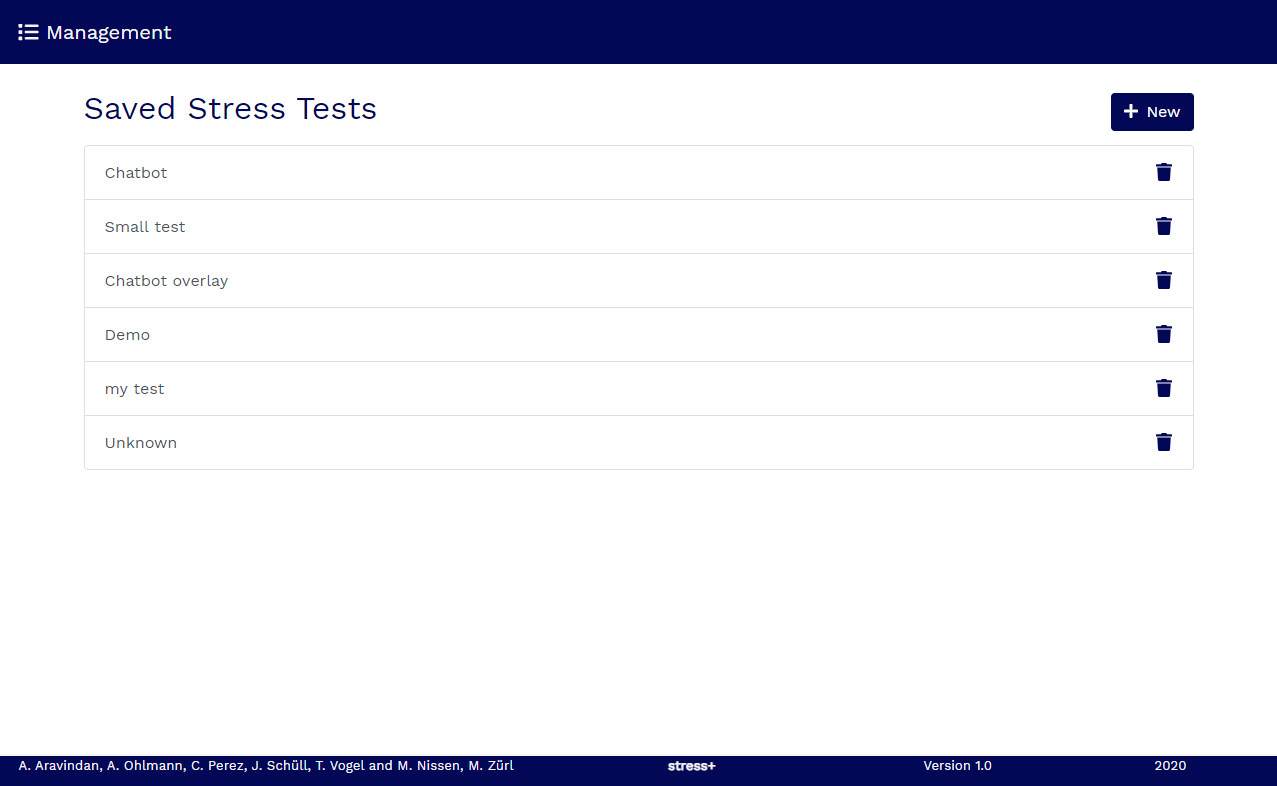
\includegraphics[width=8.5cm]{AttrakDiff/screenshot-management-page.png}
\caption{\label{mgmt-page}Management page of Stress+}
\end{figure}

The editor page is the place where the test is created. The name of the test can
be assigned using the text field on top. The available screens and overlays are
organized in the respective toolbars. The user creates a pipeline using drag and
drop. After that, each of the item's settings can be modified. The stress test
can be saved with the button ``Save settings'' at the bottom. A screenshot can be
found in figure \ref{editor-fig}.

\begin{figure}[t!]
\centering
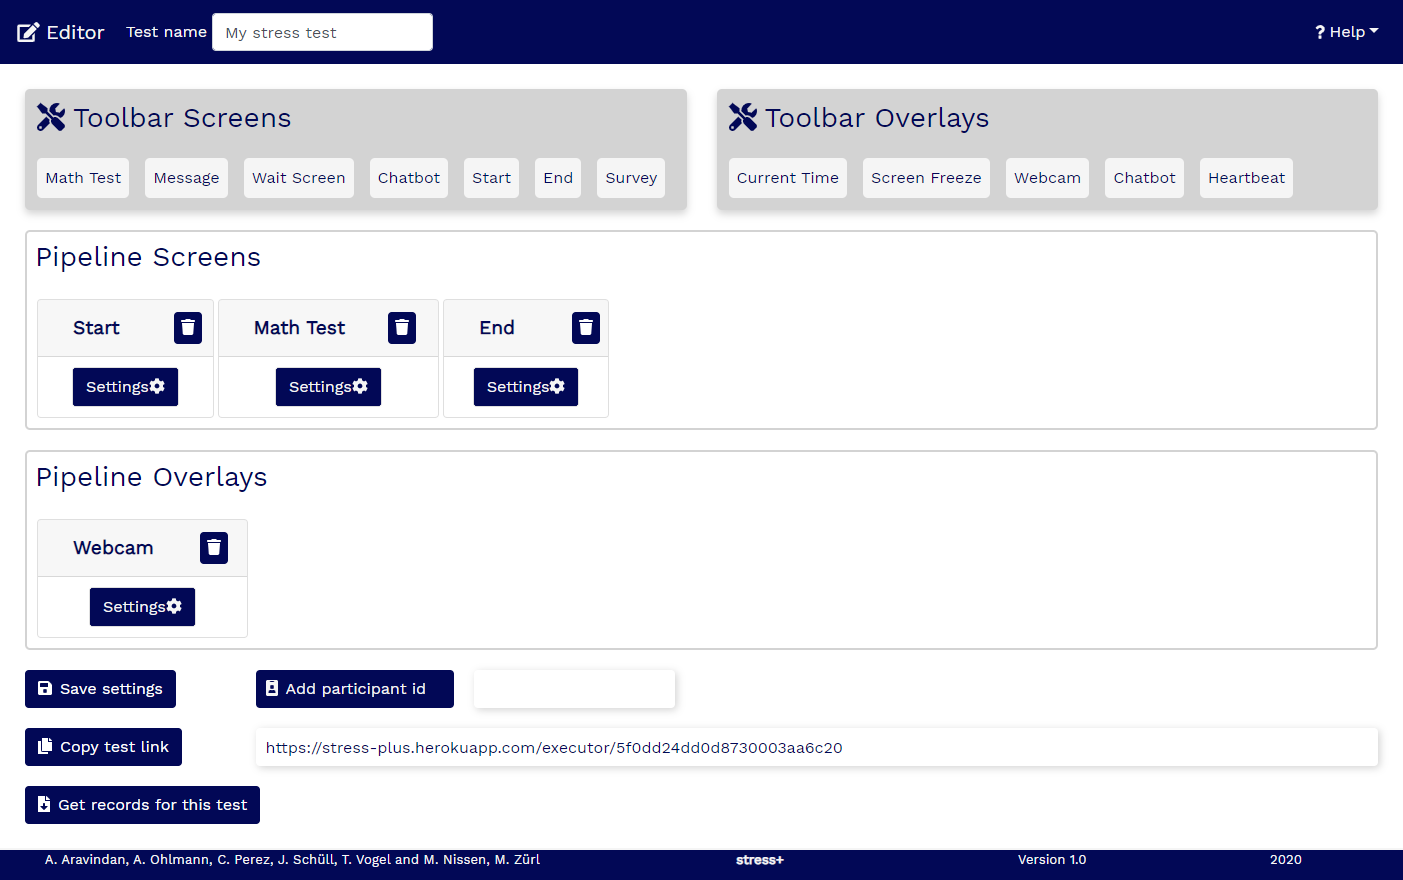
\includegraphics[width=8.5cm]{AttrakDiff/screenshot-editor-with-items.png}
\caption{\label{editor-fig}Editor page of Stress+}
\end{figure}

\subsection{AttrakDiff}
\label{sec:AttrakDiff}
AttrakDiff is built upon Hassenzahl’s model for user experience
\cite{inbook_userProduct}, illustrated in figure \ref{figure-ux}. He assumes that a
product has features that are manipulated by the designer to convey an intended
product character.

Each person who uses the product constructs a personal version of the product
character, consisting of pragmatic and hedonic qualities. This appears as
consequences, such as judgment about the product's appeal, emotional(pleasure)
and behavioral(satisfaction) consequences.

The AttrakDiff study evaluates the product character in its two groups of
attributes: pragmatic and hedonic. A product is perceived as pragmatic when it
provides effective and efficient ways to manipulate the environment. This is
strongly related to the utility and usability. A product is perceived as hedonic
if it provides stimulation, identification or provokes memories \cite{article}.

An illustrative example is the task of driving a nail. A pragmatic perspective
would be using a hammer, which does the job without much effort. From a hedonic
point of view someone might buy a certain brand to show professionalism, or
other would buy a complete set of tools to build a hammer because it is more satisfactory than just using one
\cite{inbook_userProduct}.

To assess the perceived product character, AttrakDiff measures the
attractiveness of the prototype in the format of semantic differentials,
consisting of 28 seven-step items, paired as opposite adjectives and ordered in
a scale of intensity from -3 to 3 \cite{noauthor_AttrakDiff_nodate}. It has been
shown that hedonic and pragmatic qualities are consistent and independent, and
both contribute to the attractiveness rating \cite{article}.

The ultimate goal for a product character is to have an uncompromising
combination of strong pragmatic and hedonic attributes. But most likely, both
are not in balance, which leads either to a primarily pragmatic product
(task-oriented) or primarily hedonic product (self-oriented)
\cite{inbook_userProduct}. This fact is explored in figure \ref{figure-grid}.


\begin{figure}[t!]
\centering
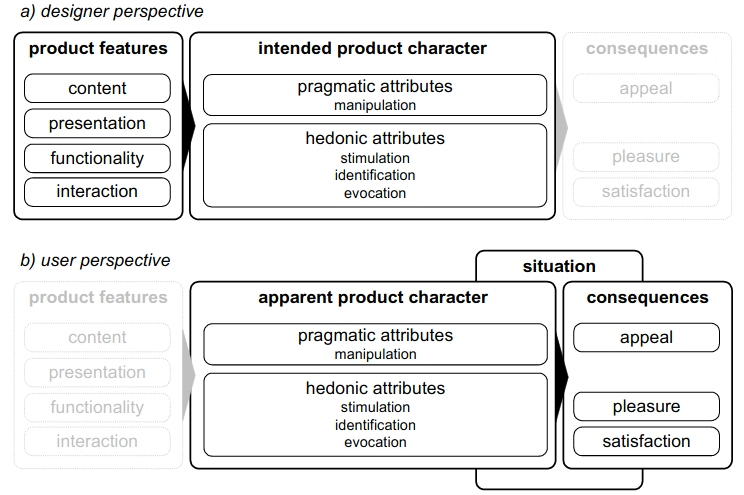
\includegraphics[width=8.5cm]{AttrakDiff/ux.jpg}
\caption{\label{figure-ux}Hassenzahl UX model \cite{inbook_userProduct}}
\end{figure}

\section{Results}
\label{sec:org605c25b}

\subsection{AttrakDiff}
\label{sec:org6acc54b}
We obtained the following results, shown in the grid view that maps hedonic
quality and pragmatic quality in figure \ref{figure-grid}. This indicates that the
product is slightly task oriented, but given the confidence region, it is close
to the desired combination of hedonic and pragmatic quality.

\begin{figure}[t!]
\centering
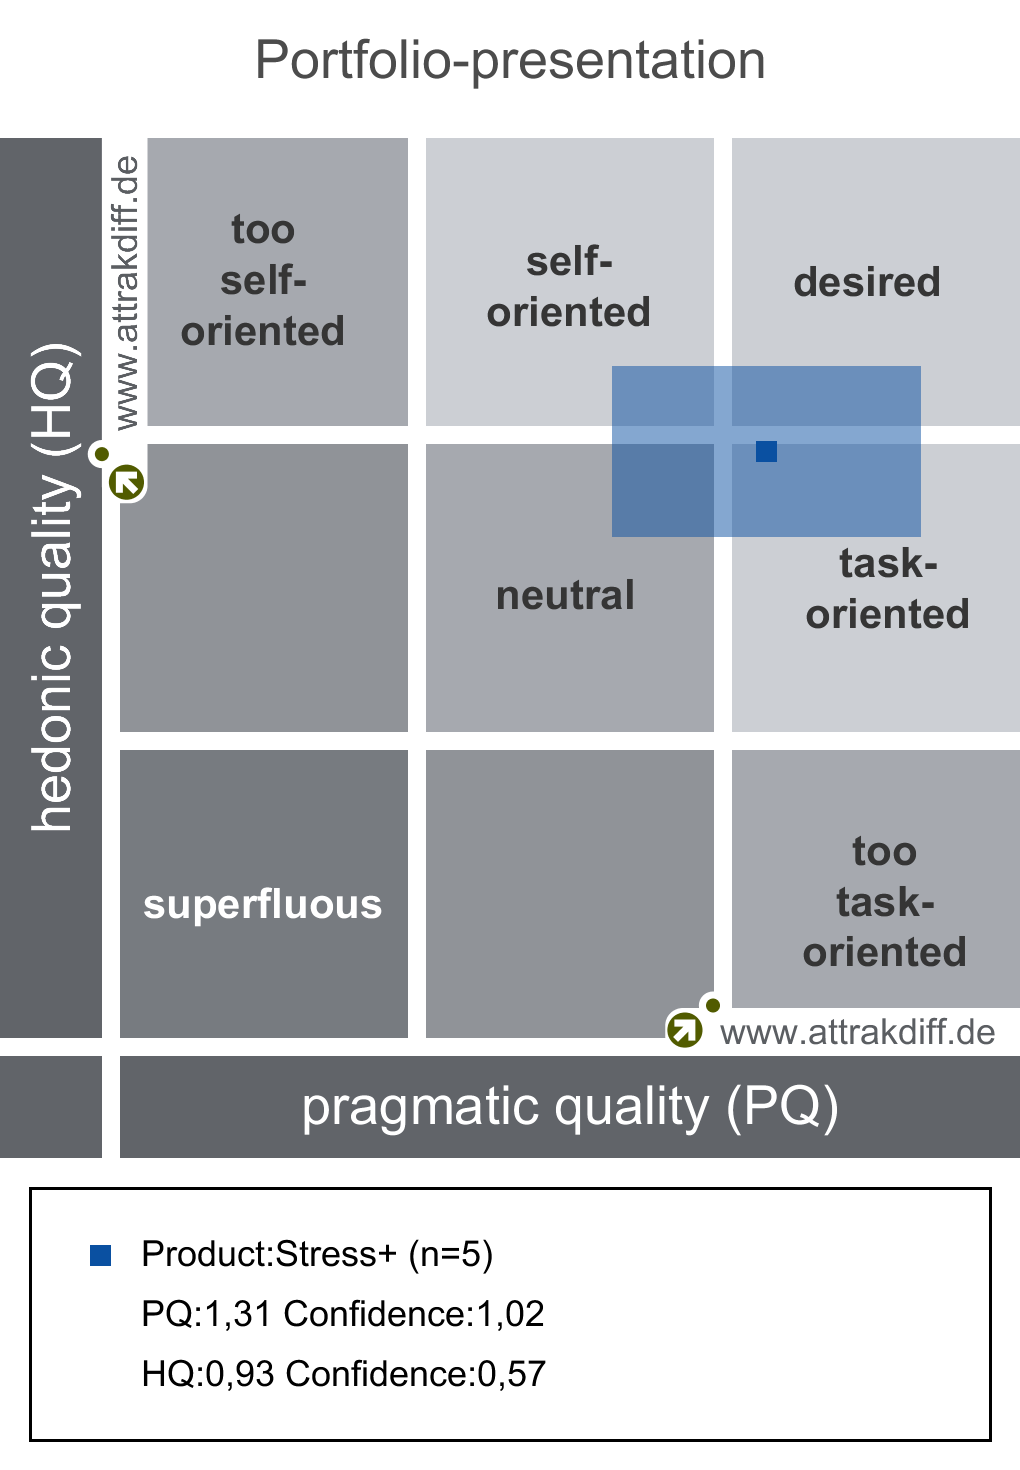
\includegraphics[width=6.5cm]{AttrakDiff/Portfolio of results.png}
\caption{\label{figure-grid}Grid view}
\end{figure}

Figure \ref{figure-word-pairs} shows the average the scale of intensity of each of
the 28 word pairs. According to it, the most important words for the pragmatic
quality are \textbf{simple} and \textbf{practical}, \textbf{presentable} for the identity hedonic
quality, \textbf{innovative} and \textbf{novel} for the stimulation hedonic quality and \textbf{good}
for the attractiveness.

\begin{figure}[t!]
\centering
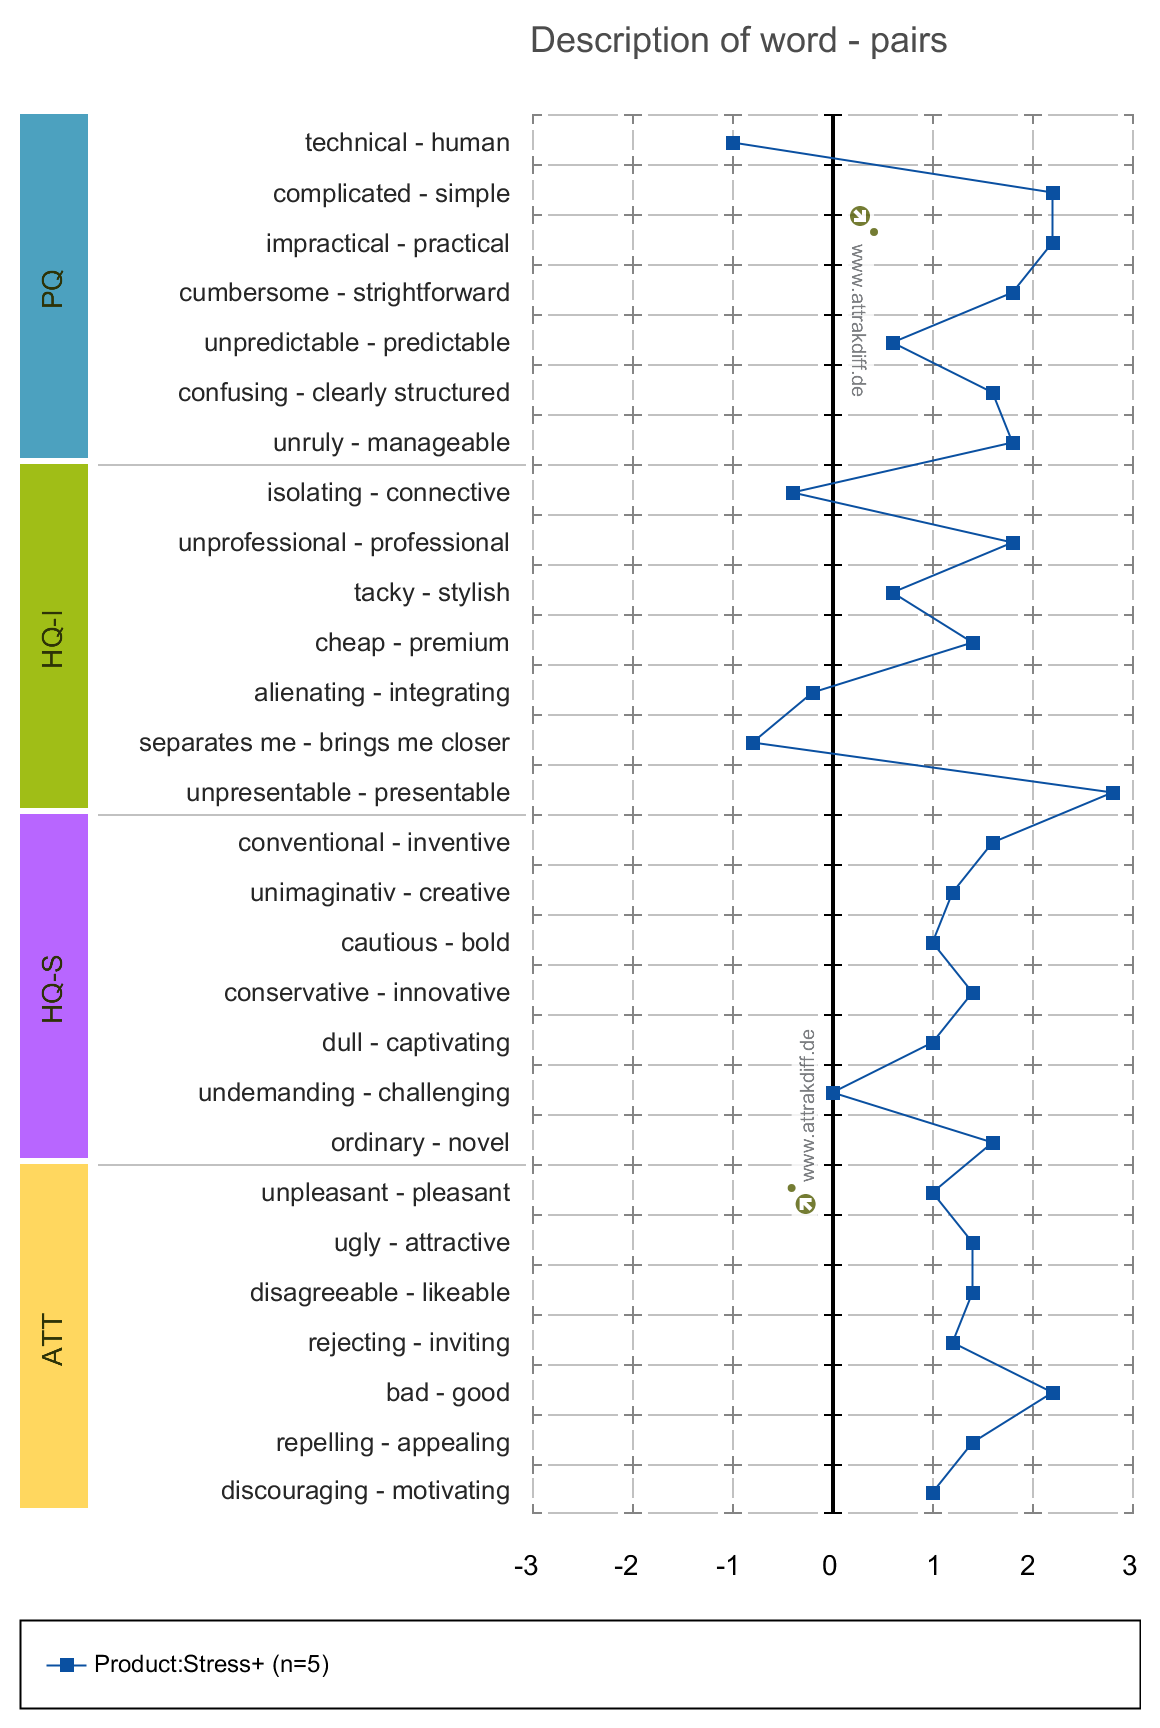
\includegraphics[width=8.5cm]{AttrakDiff/Description of word-pairs.png}
\caption{\label{figure-word-pairs}Description of word pairs}
\end{figure}

The diagram of average values shown in figure \ref{figure-avg-vals} shows the
averages for each quality. All the scores are above zero, which means in all
cases they evoke positive emotions. It also shows that Stress+ performs better
in the pragmatic quality than in the hedonic quality.

\begin{figure}[t!]
\centering
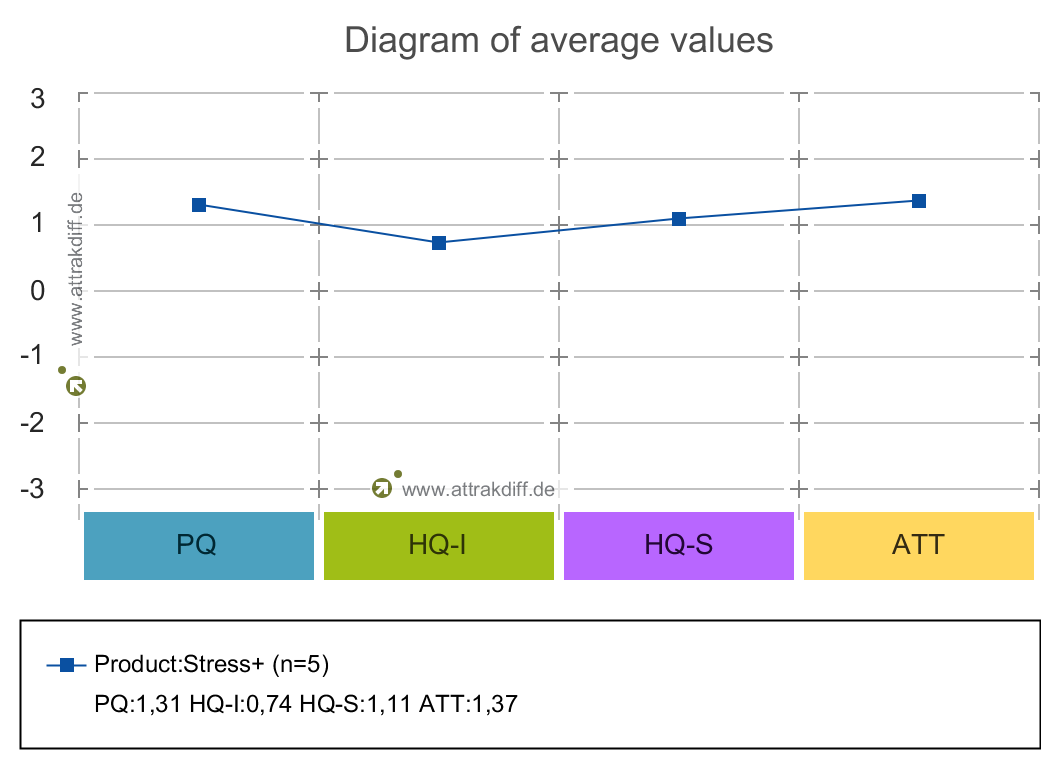
\includegraphics[width=7.5cm]{AttrakDiff/Diagram of average values.png}
\caption{\label{figure-avg-vals}Diagram of average values}
\end{figure}

\subsection{Performance of the participants}
\label{sec:orgbe6298c}
All the participants were able to follow the instructions and finish the task
successfully with a short explanation about the application.

Based on the observations of the performance of the participants during the
tasks assigned in the study session, these are some of the most important points
to improve:
\begin{itemize}
\item The difference between a generic \texttt{Message} screen and the \texttt{End} screen or
\texttt{Start} screen was not intuitive at the beginning for some of the
participants.
\item The \texttt{chatbot} settings interface is not intuitive. It was not clear to the
participants that the test expects a reply from the user in between each
custom message.
\item It could be useful to add auto save functionality: one of the participants
accidentally closed the screen without saving for some time and most of the
settings were deleted.
\end{itemize}

The feedback received for improvement is summarized in the following points:
\begin{itemize}
\item Order the saved tests in the management page by creation date, with the newest
at the top.
\item The dark blue color for the buttons make them more prominent than they should
be.
\item Reduce the size of the settings button.
\item Chatbot functionality is still not realistic enough to be effectively used in
a real stress test.
\end{itemize}

\section{Discussion}
\label{sec:discussion}
The current prototype has a good performance in terms of the user experience and
usability, based on the quantitative results obtained from the AttrakDiff test
and the comments received during the sessions.


Based on figure \ref{figure-grid}, it is possible to conclude that the product is
near the desired value combination for hedonic and pragmatic qualities . This
means the product is useful and at the same time likeable. The slightly higher
choice of a stronger pragmatic qualities by the participants can be explained by
the nature of the interface, being more technical in principle, mainly focused
on the creation and modification of a stress test.

The results in figure \ref{figure-grid} lead to the conclusion that the feeling of
interactivity with the application (hedonic interactive quality) was the lowest
of the evaluated qualities, in part influenced by its technical nature, even if
the drag and drop feature should have improved this aspect.To be more specific,
the majority of low scores in the word pairs belong to the hedonic interactive
quality, as observed in figure \ref{figure-word-pairs}. Words such as \textbf{isolating},
\textbf{alienating} and \textbf{separates me} were preferred over \textbf{connecting}, \textbf{integrating}
and \textbf{brings me closer} respectively. One way to improve the interaction would be
to provide a wizard that guides the user through the test creation and some
settings modifications. Nevertheless, given that the Editor page is purely
technical-oriented, it is not necessarily negative that it evokes these feelings
in the participants.

The use of AttrakDiff facilitates the comparison with future iterations of the
application, which is even a built-in option of the methodology. Another reason
to choose it over other tools such as SUS (System Usability Scale) is explained
by its holistic view which not only includes usability evaluation in the form of
pragmatic qualities, but also emotional aspect as hedonic qualities in a single
questionnaire. The test is also intuitive and provides little burden for the
participants. It is also easy to put in practice in a remote study such as this
case. Besides, its results have a clear and fast interpretation.

The feedback given by the participants was mainly in the direction that Stress+
is a considerable improvement in comparison to the MIST software they have used
before. It was also easy for them to get started using the \texttt{Editor} page and
therefore they could focus on more specific details of the user interface during
the study.

\section{Summary and outlook}
\label{sec:org8db07b4}

Stress+ is a web application that builds upon the MIST as a tool to help
researchers study in the laboratory how stress is related to illness. It
achieves that by providing more features and enhancing the user experience of
the researchers with the application. After performing a user experience study
with the help of the AttrakDiff system, we discovered that Stress+ is already
addressing some of the pain points of the previous protocols have, and also know
in which direction to apply changes to improve how the users interact with it.

The next step is to apply changes to address the comments from the participants
and the shortcomings observed after they performed their tasks and then use the
same analysis tools to evaluate the user experience and usability of the new
iteration of the prototype. By using the results obtained in this first study as
a baseline, it would be possible to judge whether the changes are in the right
direction and where they impact the most.

\bibliography{my}

\bibliographystyle{IEEEtran}


\newpage
\section{Appendix}
\label{sec:orgec501f8}

\subsection{Tasks performed by the participants}
\label{sec:protocol}
\textbf{Task 1}

\begin{enumerate}
\item Create a new test with a custom name

\item Add the following screens:
\begin{enumerate}
\item Wait screen
\item Start screen
\item Math test with control activated, difficulty 1
\item Message to indicate a new test
\item Math test, sound activated, 40 seconds, difficulty 4
\item Chat bot. Create a 2-step dialogue asking about performance
\item Math test. Choose your parameters
\item End message
\end{enumerate}

\item Save the test
\end{enumerate}


\textbf{Task 2}

\begin{enumerate}
\item Save the test
\item Close the page
\item Use link to open again
\item Enter to your saved test
\item Get the link and copy it in the zoom chat.
\end{enumerate}
\end{document}
